\begin{figure}[htb]
\centering
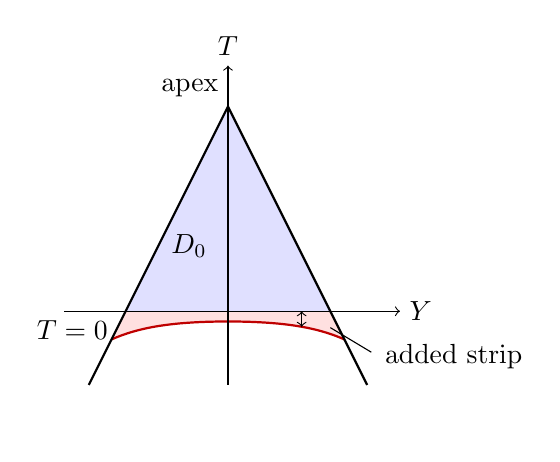
\begin{tikzpicture}[scale=5.2]
 \fill[blue!12] (-.25,0)--(.25,0)--(0,.5)--cycle;
 \begin{scope}
  \clip (-.4,-.3)--(.4,-.3)--(0,.5)--cycle;
  \fill[red!12] (-.34,0)--(.34,0)
    -- plot[domain=.34:-.34,samples=80]
       (\x,{-.025-.3*\x*\x-3*\x*\x*\x*\x}) -- cycle;
  \draw[red!75!black,thick,domain=-.34:.34,samples=80]
    plot (\x,{-.025-.3*\x*\x-3*\x*\x*\x*\x});
 \end{scope}
 \draw[thick] (-.34,-.18)--(0,.5)--(.34,-.18);
 \draw[dashed] (-.25,0)--(.25,0);
 \draw[->] (0,-.18)--(0,.60) node[above] {$T$};
 \draw[->] (-.40,0)--(.42,0) node[right] {$Y$};
 \node[below left] at (-.27,0) {$T=0$};
 \node at (-.095,.16) {$D_0$};
 \node[above left] at (0,.5) {apex};
 \draw[<->] (.18,0)--(.18,-.038);
 \node[right] at (.36,-.11) {added strip};
 \draw[thin] (.35,-.10)--(.25,-.04);
\end{tikzpicture}
\caption{Schematic intercept domain for the first family. The blue
triangle is the unperturbed domain $D_0$; the red strip extends it
below $T=0$. The padded lower boundary ends at the unchanged wedge
walls. Its actual equation is $T=-\epsilon^2P(Y)-q$; the padding is
exaggerated here, and the walls continue below the displayed portion.}
\label{c:fig-equality}
\end{figure}
